\documentclass[11pt]{article}
% -- Formato
\input{formato}

% -- Paquetes adicionales
\usepackage{amsmath,amssymb}
\usepackage{enumitem}
\usepackage{float}



% -- Comandos extra


% -- Datos
\title{Manual de operação: ComMarker B6 MOPA Fiber Laser Engraver}
\author{Henrique de O. Bernardes}
\affil{}
\date{\today}

% --- Archivo de bibliografía
\addbibresource{ref.bib}

%%%%%%%%%%%%%%%%%%%%%%%%%%%%%%%%%%%%%%%%
\begin{document}

%%%%%%%%%%%%%%%%%%%%%%%%%%%%%%%%%%%%%%%%
\maketitle
\thispagestyle{fancy}


\section{Identificação do Documento}
\textbf{Equipamento: ComMarker B6 MOPA Fiber Laser Engraver}\\
\textbf{Categoria: Gravadora}\\

\subsection{Controle de Revisões}
\begin{center}
\begin{tabular}{|c|c|p{8cm}|}
\hline
\textbf{Versão} & \textbf{Data} & \textbf{Descrição} \\
\hline
1.0 & 07/02/2026 & Manual técnico inicial \\
\hline
% Adicione novas linhas aqui
% 1.1 & 01/01/2025 & Atualização de conteúdo \\
% \hline
\end{tabular}
\end{center}


\section{Objetivo}
O objetivo deste manual de operação é fornecer orientações para o uso adequado da \textbf{ComMarker B6 MOPA Fiber Laser Engraver}, assegurando que o operador seja capaz de operar o equipamento de forma segura, eficiente e com alto padrão de qualidade. Este documento busca ainda minimizar riscos associados à operação do laser, prevenir danos ao equipamento e aos materiais processados, além de auxiliar na identificação e solução de possíveis falhas. Adicionalmente, o manual tem como finalidade padronizar procedimentos, facilitar o treinamento de novos usuários e garantir o melhor desempenho do sistema ao longo de sua vida útil.
\section{Visão Geral Da Gravadora}
A ComMarker B6 MOPA Fiber Laser Engraver é uma gravadora a laser de fibra com potência de 60W. O equipamento utiliza tecnologia de laser do tipo MOPA (Master Oscillator Power Amplifier), operando  no comprimento de onda de 1064 nm, sendo possível realizar gravações, marcações e cortes em metais e alguns materiais não metálicos. Dentre os materiais principais que podem ser gravados de acordo com a fabricante estão:
\begin{itemize}
  \item Cobre
  \item Alumínio
  \item Acrílico
  \item Prata
  \item Aço inoxidável
  \item Plástico
\end{itemize}
\begin{figure}
  \begin{center}
    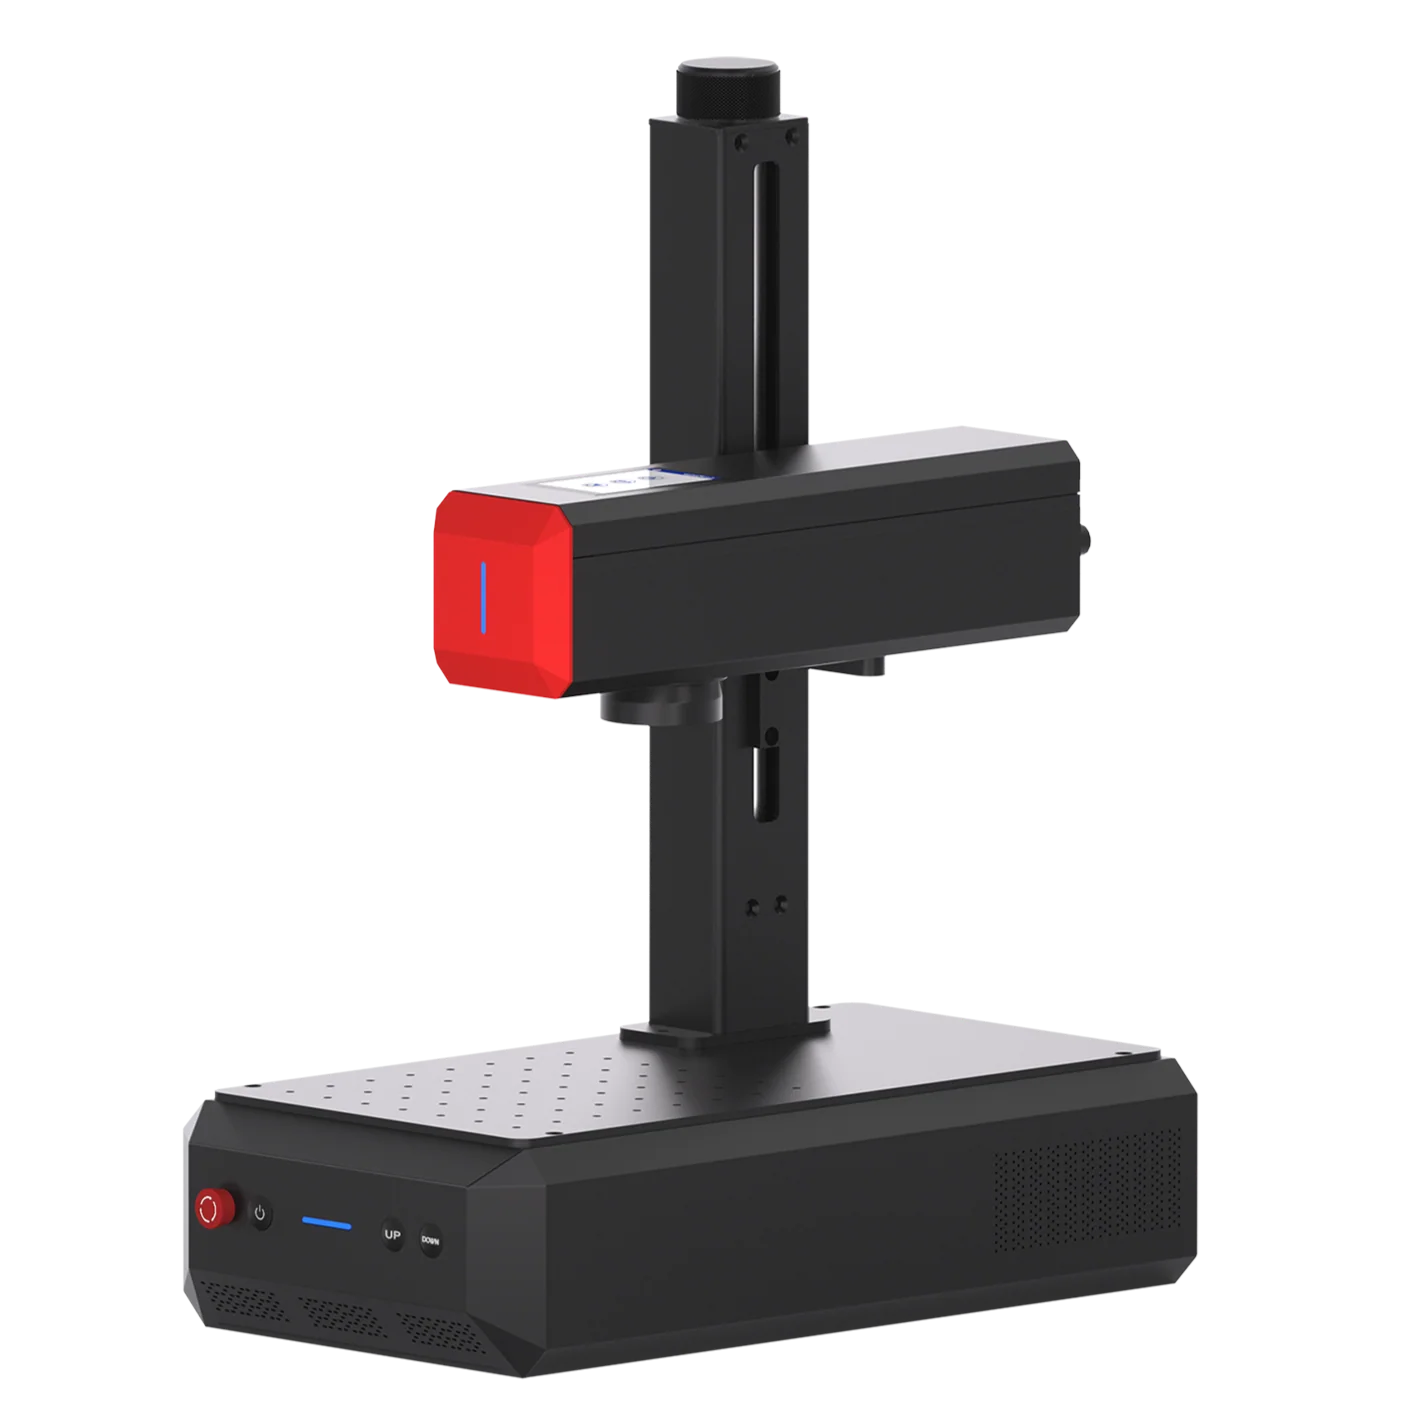
\includegraphics[width=0.45\textwidth]{figures/B6Mopa.jpg}
  \end{center}
  \caption{ComMarker B6 MOPA Fiber Laser Engraver}\label{fig:}
\end{figure}

\section{Identificação dos Componentes}
\begin{figure}[h]
  \centering
  \begin{minipage}{0.50\textwidth}
    \centering
    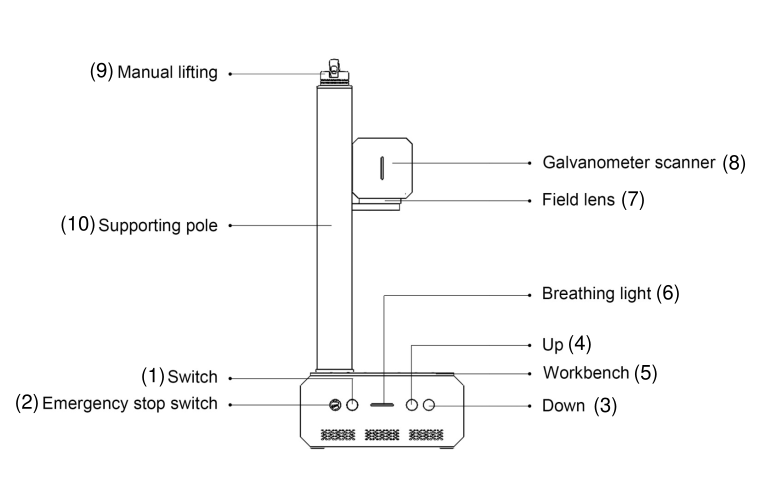
\includegraphics[width=\linewidth]{figures/frenteB6Anotada.png}
    \caption{Visão frontal da gravadora}
  \end{minipage}\hfill
  \begin{minipage}{0.50\textwidth}
    \centering
    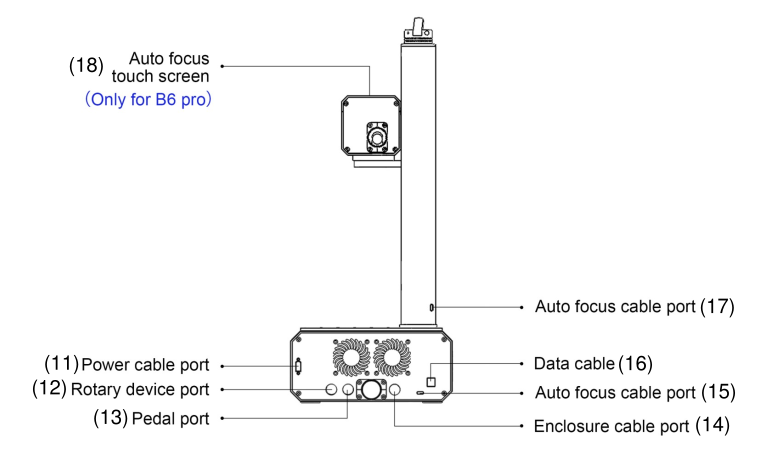
\includegraphics[width=\linewidth]{figures/trasB6Anotada.png}
    \caption{Visão traseira da gravadora}
  \end{minipage}
\end{figure}
\begin{enumerate}
  \item Switch: Botão de liga/desliga;
  \item Emergency stop switch: Chave de parada de emergência;
  \item Down: Movimentação do conjunto do laser para baixo;
  \item Up: Movimentação do conjunto do laser para cima;
  \item Workbench: Bancada/Superfície de trabalho;
  \item Breathing light: Luz indicadora de estado(ligado/desligado);
  \item Field lens: Lente de campo;
  \item Galvanometer scanner: Scanner galvanometro;
  \item Manual lifting: Elevadora manual do conjunto laser;
  \item Supporting pole: Coluna de suporte;
  \item Power cable port: Porta do cabo de alimentação;
  \item Rotary device port: Porta do eixo rotativo;
  \item Pedal port: Porta para pedal;
  \item Enclosure cable port: Porta para cabos de fora do gabinete;
  \item Auto focus cable port: Porta para cabo do foco automático;
  \item Data cable: Cabo de dados(USB);
  \item Auto focus cable port: Porta para cabo do foco automático;
  \item Auto focus touch screen: Tela para foco automático.
\end{enumerate}
 
\section{Parâmetros de Impressão Recomendados}
Os parâmetros variam a depender do material. Para materiais diversos, encontra-se nas referências um GitHub com um conjunto de parâmetros para materiais diversos feito pela própria ComMarker. Consta, também, um conjunto de parâmetros voltados para placas de cobre. 
\newpage
\section{Fluxograma Operacional do Processo}
Na imagem \ref{fig:fluxogramaOperacionalGravadora} vemos o fluxograma operacional do processo de gravação:
\begin{figure}[!h]
  \begin{center}
    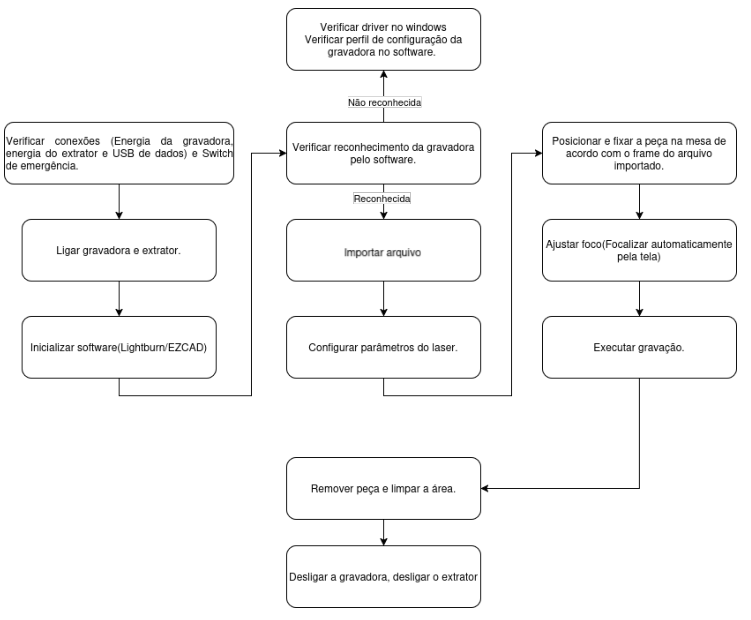
\includegraphics[width=0.75\textwidth]{figures/fluxograma.png}
  \end{center}
  \caption{Fluxograma operacional da gravadora}\label{fig:fluxogramaOperacionalGravadora}
\end{figure}


\section{Verificando Drivers}
Antes de qualquer coisa, deve-se instalar o driver da gravadora no computador que será utilizado para envio dos arquivos para gravação. Para isso, conecte o USB de dados da gravadora no computador e verifique no Gerenciador de Dispositivos do Windows por um dispositivo com um dos nomes: "USBLMCV2", "USBLMCV4" ou "Unknown Device", podendo ser encontrados nas abas "Other devices" ou "Universal Serial Bus devices". 
Agora, deve-se atualizar o driver do dispositivo para ser reconhecido adequadamente pelo Windows. Foi observado que, em algumas instâncias, o Windows automaticamente atualiza o driver e reconhece a gravadora sem procedimentos extras. Se esse não for o caso, deve-se atualizá-lo manualmente. Para isso, clique com o botão direito em cima do nome do dispositivo e em "Update driver", então, selecione "Browse my computer for drivers". Deve-se encontrar a pasta que contem o driver adequado para a versão de Windows sendo utilizada na pasta "driver" dos arquivos da gravadora. Estes passos são mostrados na figura \ref{fig:driverB6} e \ref{fig:driversFolderB6}
\begin{figure}[!h]
  \begin{center}
    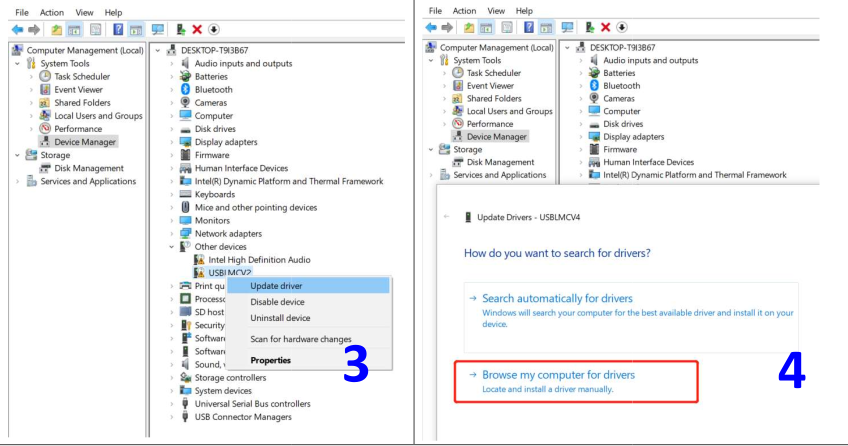
\includegraphics[width=0.95\textwidth]{figures/driverB6.png}
  \end{center}
  \caption{Atualizando o driver da gravadora}\label{fig:driverB6}
\end{figure}
\begin{figure}[!h]
  \begin{center}
    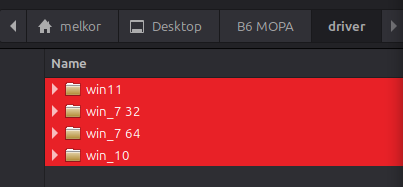
\includegraphics[width=0.35\textwidth]{figures/driversFolderB6.png}
  \end{center}
  \caption{Pasta drivers contendo os drivers para cada versão de Windows}\label{fig:driversFolderB6}
\end{figure}

\newpage
\section{Procedimento Operacional}
Antes de ligar a gravadora, é necessário verificar se os cabos de energia da gravadora e do extrator estão ligados e conectar o cabo USB de dados da gravadora no computador a ser utilizado. Feito isso e verificada a conexão adequada dos cabos, liga-se a gravadora(a partir do \textit{Switch} de ligar) e a extratora(girando o botão de potência para a potência requerida para o processo).

Com os aparelhos ligados e o cabo USB de dados da gravadora conectado ao computador, inicializa-se o software de preferência, podendo ser utilizado tanto o \textit{Lightburn} quanto o \textit{EZCAD}. Este manual utiliza por base o \textit{Lightburn} por ter uma interface mais clara e objetiva, facilitando o uso. 
Ao inicializar o software, caso for a primeira vez, deve-se configurar a gravadora para ser reconhecida pelo software. Para isso, logo ao abrir o software, clica-se em "Find My Laser"

\begin{figure}
  \begin{center}
    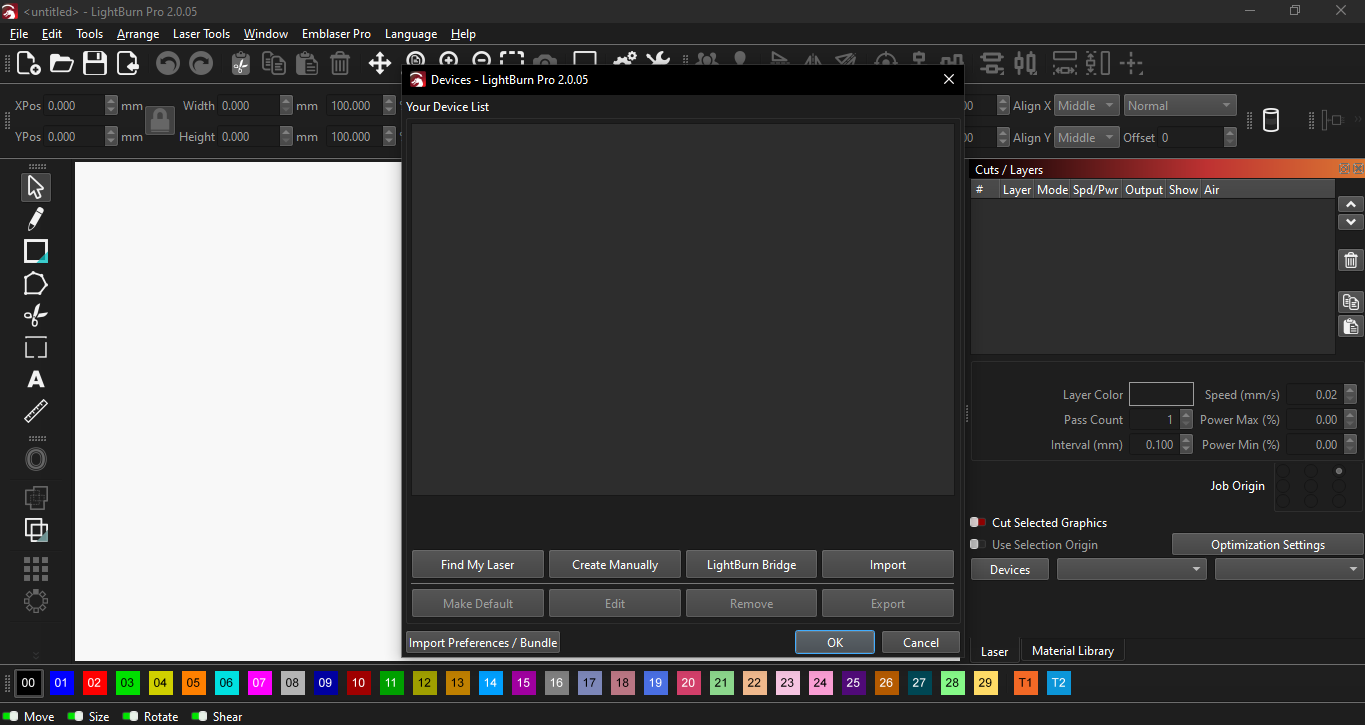
\includegraphics[width=0.95\textwidth]{figures/settingUp/findMyLaser.png}
  \end{center}
  \caption{Find My Laser}\label{fig:}
\end{figure}

Ao encontrar o laser, adiciona-se o laser ao LightBurn clicando em \textit{Add Device}.

\begin{figure}
  \begin{center}
    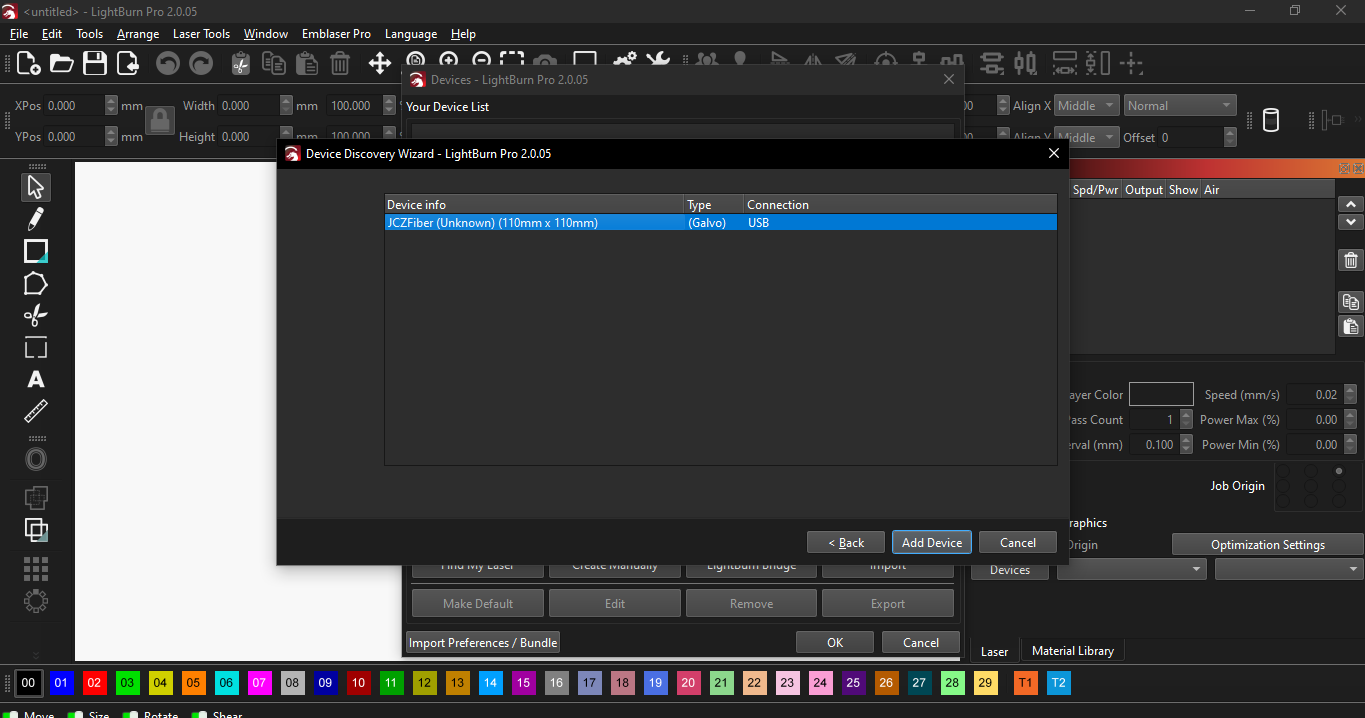
\includegraphics[width=0.95\textwidth]{figures/settingUp/laserFound.png}
  \end{center}
  \caption{Laser Found}\label{fig:}
\end{figure}

\begin{figure}
  \begin{center}
    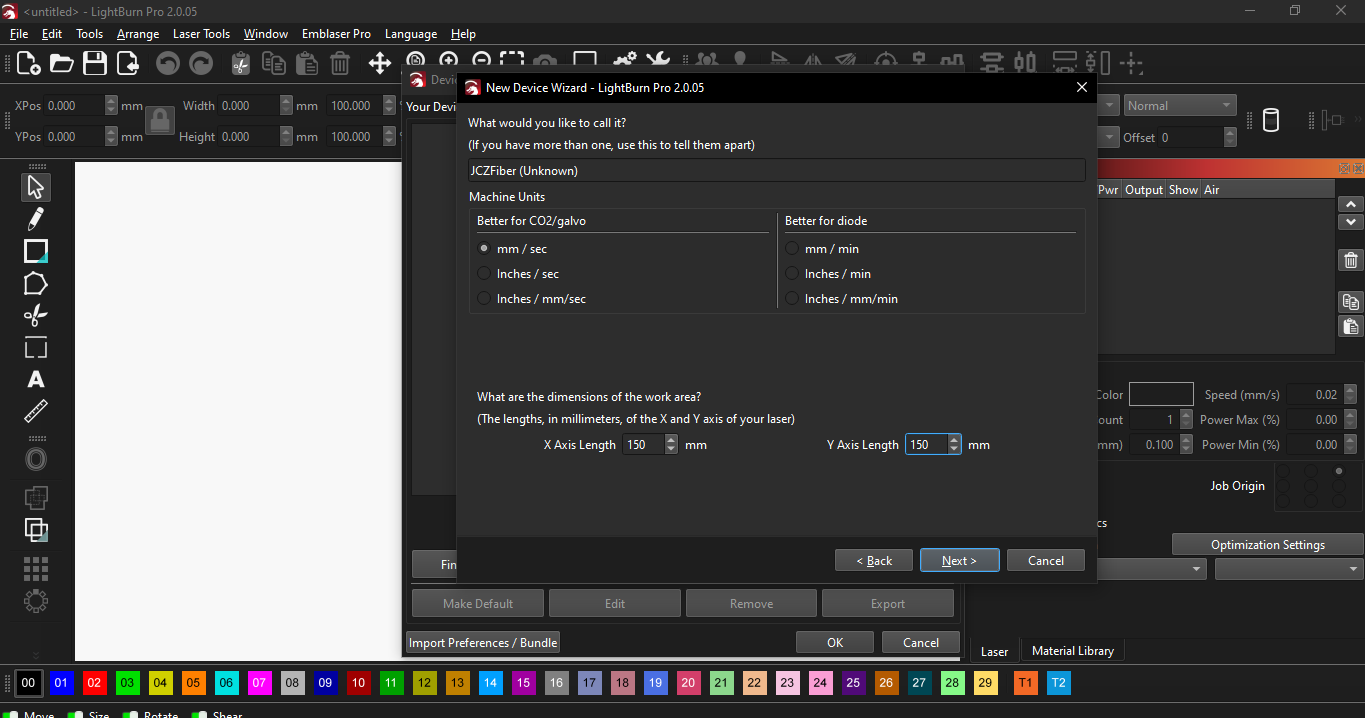
\includegraphics[width=0.95\textwidth]{figures/settingUp/150150.png}
  \end{center}
  \caption{Laser Dimensions}\label{fig:}
\end{figure}

Precisamos então carregar o arquivo de configuração do EZCad:

\begin{figure}
  \begin{center}
    \includegraphics[width=0.95\textwidth]{figures/settingUp/EZCadConfigFile.png}
  \end{center}
  \caption{EZCad Config File}\label{fig:}
\end{figure}

\begin{figure}
  \begin{center}
    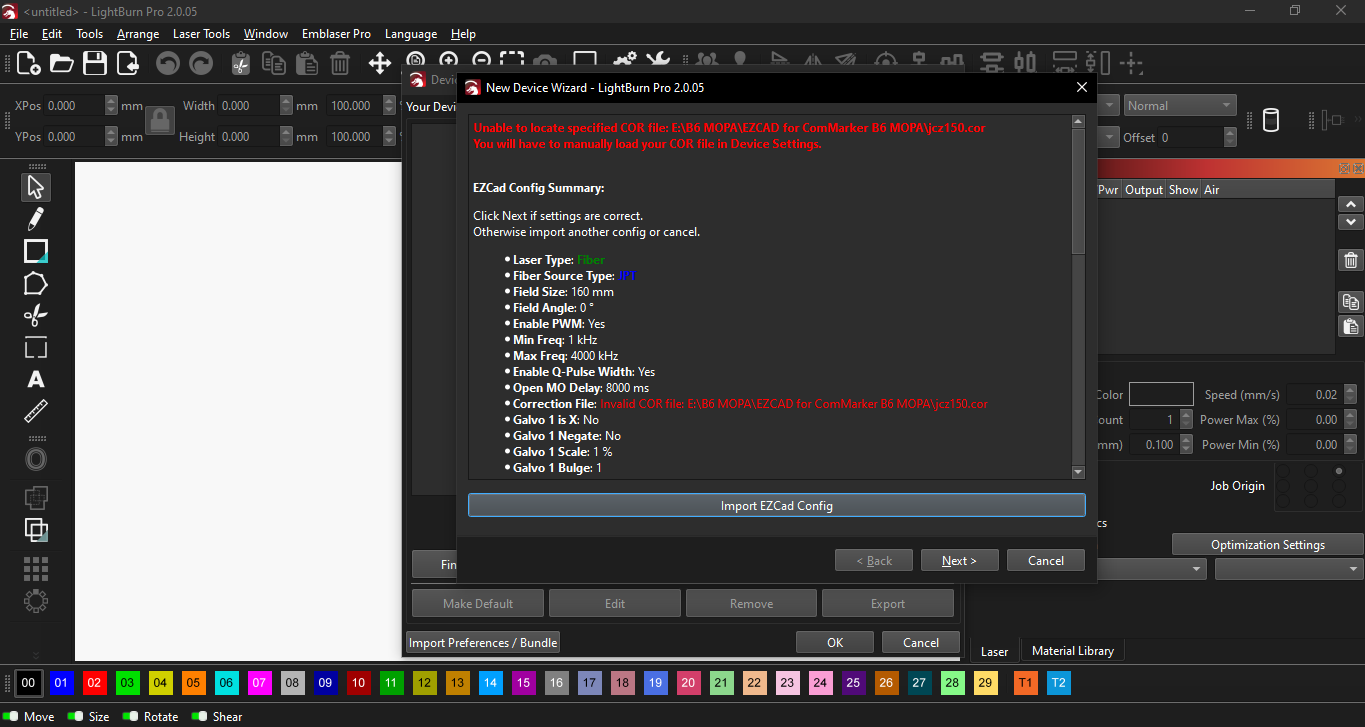
\includegraphics[width=0.95\textwidth]{figures/settingUp/Step1done.png}
  \end{center}
  \caption{EZCad Config File}\label{fig:}
\end{figure}

Feito isso, o primeiro passo foi completo.

Por fim, acessamos Device Settings e ajustamos os parâmetros do Galvo 1 e Galvo 2 para os valores mostrados na figura \ref{fig:parametros}

\begin{figure}[!h]
  \begin{center}
    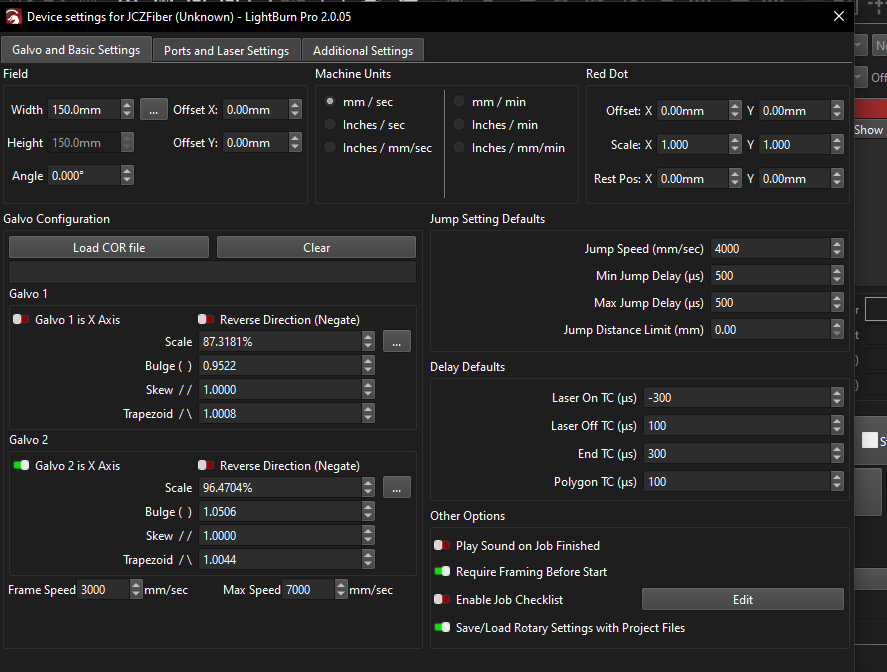
\includegraphics[width=0.75\textwidth]{figures/settingUp/paramsDevice.png}
  \end{center}
  \caption{Parâmetros de Calibração}\label{fig:parametros}
\end{figure}

\begin{figure}[!h]
  \begin{center}
    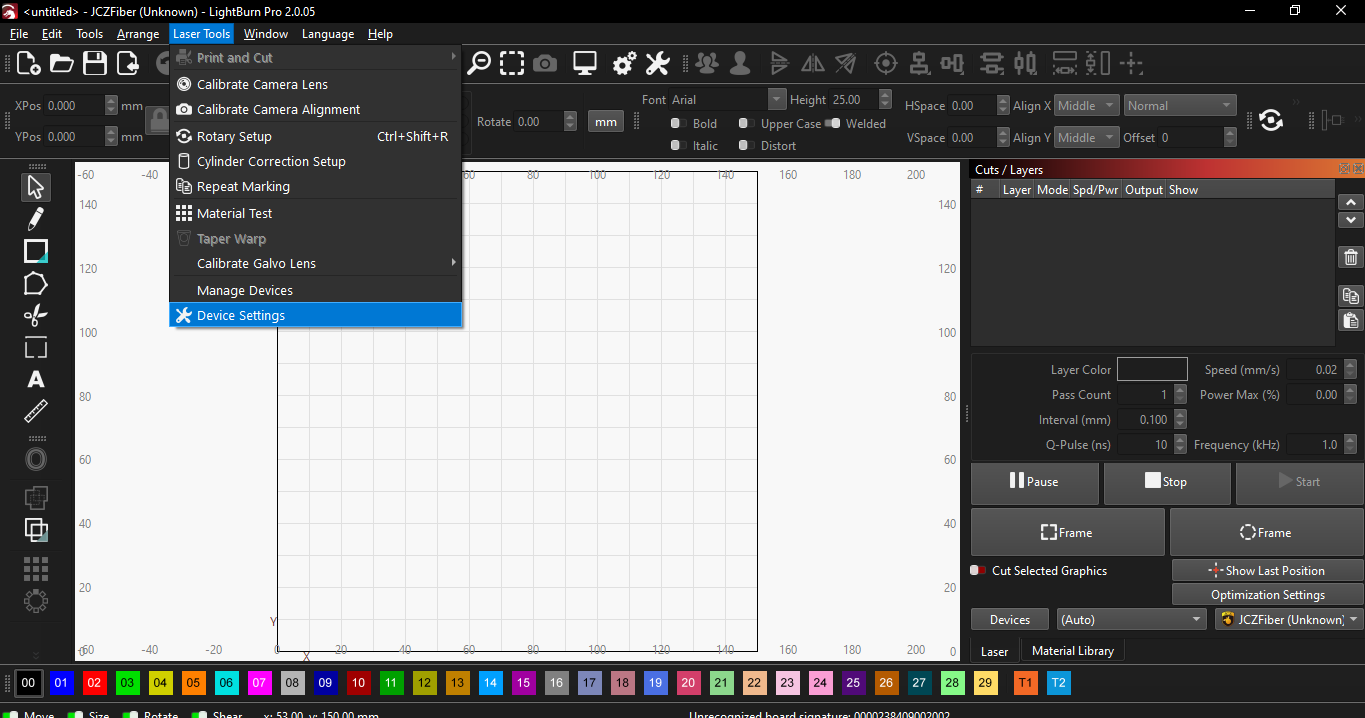
\includegraphics[width=0.95\textwidth]{figures/settingUp/deviceSettings.png}
  \end{center}
    \caption{Device Settings}\label{fig:}
\end{figure}



\section{Checklist de Pré-Impressão}
Ante da impressão existem alguns pontos a serem assegurados:

\begin{enumerate}
  \item Se a lente da gravadora está focalizada(figura \ref{fig:foco}). Ao verificar que a lente não está focada por meio do aviso, basta apertar em Auto para focalizar; 
  \item Se a lente está tampada. Caso sim, basta retirar a tampa;
  \item Se o material a ser gravado está no mesmo nível do foco da lente. Se não, deixe-o no mesmo nivel, caso contrario os parâmetros de gravação não terão o resultado desejado;
  \item Se o extrator de fumaça está ligado e encaixado no furo traseiro do gabinete one a gravadora fica dentro;
  \item Se os parâmetros sendo utilizados para gravação estão adequados para o material e finalidade;
  \item Se o switch de parada de emergência está destorcido(permitindo o funcionamento da gravadora).  
\end{enumerate}


\begin{figure}[!h]
    \centering  
    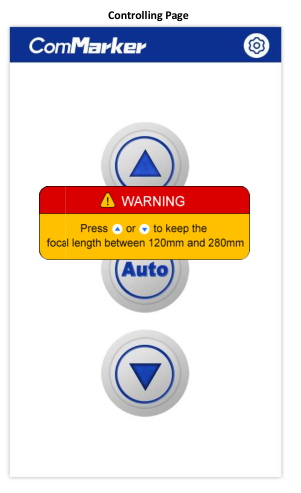
\includegraphics[width=0.3\textwidth]{figures/checkBefore/foco.png}
    \caption{Aviso da lente não focalizada.}
    \label{fig:foco}
\end{figure}
 
\section{Calibração}
Se for percebido que as dimensões do que é medido em software e o que é impresso estão distintas e/ou a gravação está espelhada, realiza-se o \textit{9 Point Correction}. O passo a passo é dado ao longo da calibração.
\begin{figure}[!h]
    \centering
    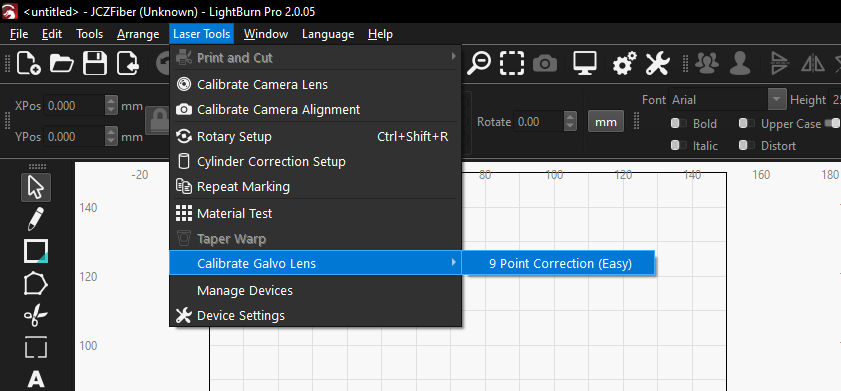
\includegraphics[width=0.5\textwidth]{figures/calibrating.png}
    \caption{Menu de calibração}
    \label{fig:label}
\end{figure}

Caso queira calibrar ela sem utilizar esta opção, é possível gravar uma geometria com dimensões conhecidas, medir os eixos x e y fisicamente pós impressão, e ajustar por meio da opção \textit{Calibrate Axis} disponível no menu \textit{Device Settings}(figura \ref{fig:calib2})

\begin{figure}[!h]
    \centering
    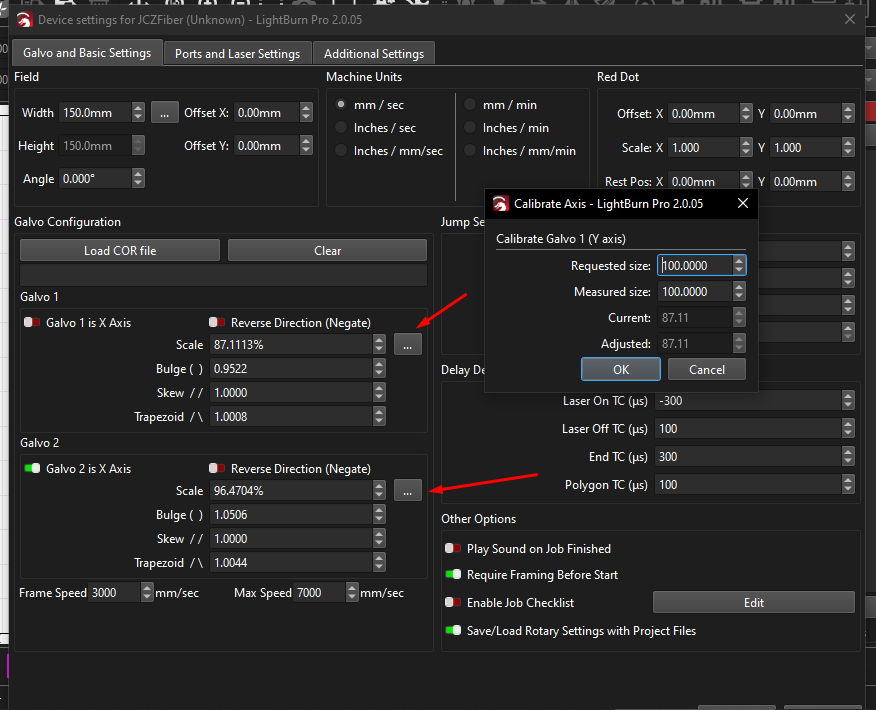
\includegraphics[width=0.4\textwidth]{figures/calibrating2.png}
    \caption{Calibração manual}
    \label{fig:calib2}
\end{figure}



\section{Início da Impressão}
Para a gravação de uma geometria em DXF, importa-se a geometria e, antes de gravar, deve ser verificado se o que será gravado está de acordo com o que é esperado por meio da ferramenta "Preview":

\begin{figure}[H]
    \centering
    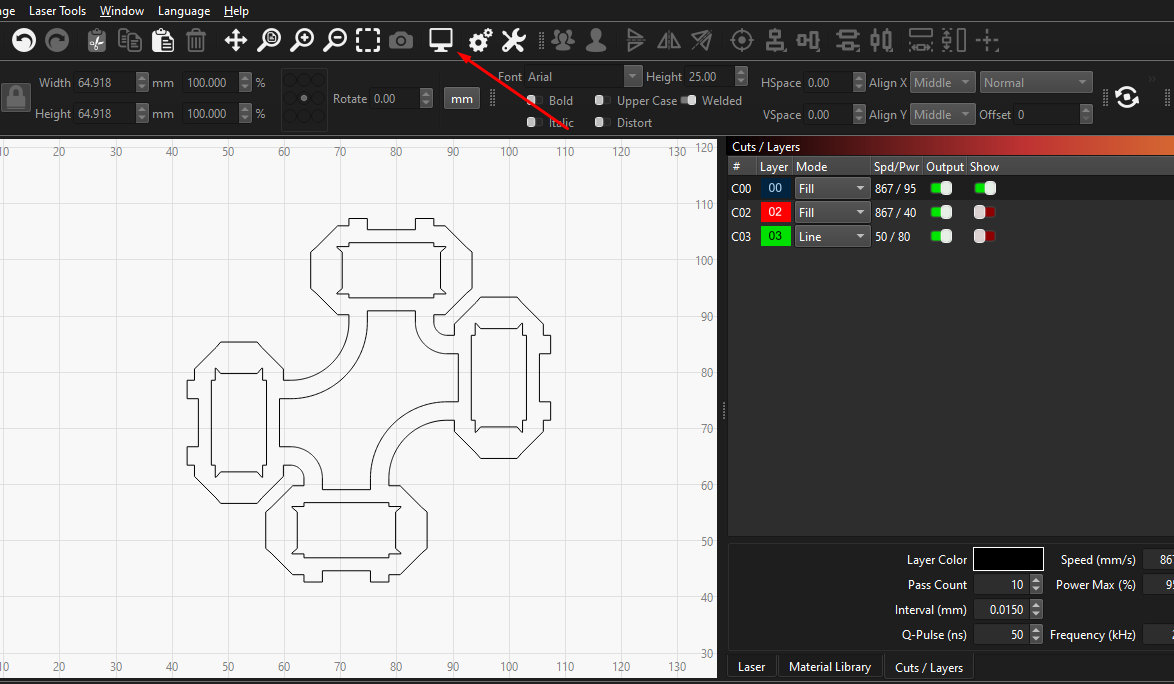
\includegraphics[width=0.6\textwidth]{figures/preview.png}
    \caption{Preview da geometria a ser gravada.}
    \label{fig:label}
\end{figure}

Com as camadas no modo Fill, observa-se que o formato da geometria em sí será gravado:

\begin{figure}[H]
    \centering
    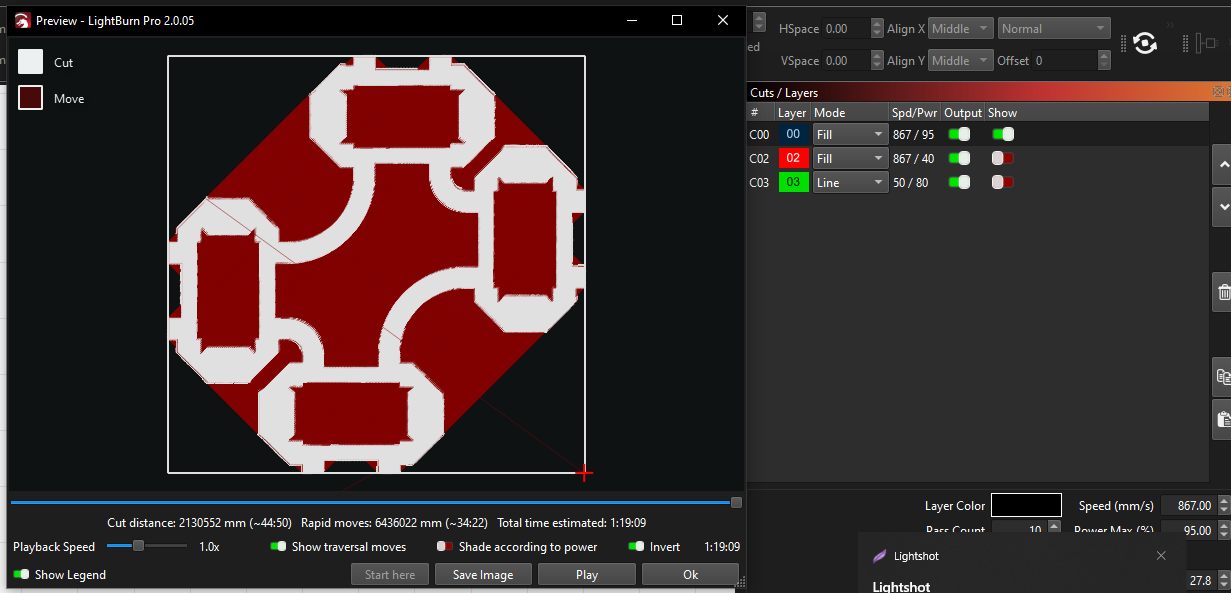
\includegraphics[width=0.6\textwidth]{figures/fillMode1.png}
    \caption{}
    \label{fig:label}
\end{figure}


Contúdo, caso queira inverter essa gravação(remover ao redor da geometria), basta criar uma geometria (na mesma camada!!) que englobe toda a geometria original, como um quadrado. Dessa forma, a gravação é invertida:


\begin{figure}[H]
    \centering
    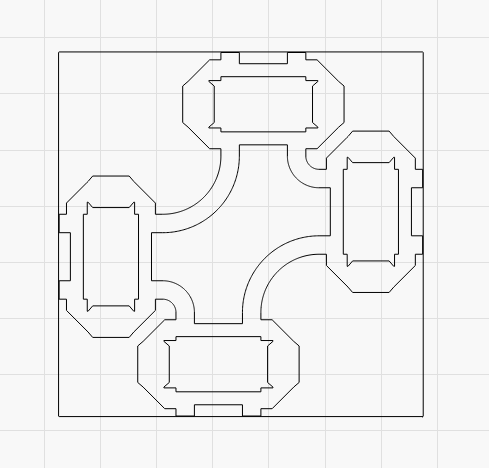
\includegraphics[width=0.6\textwidth]{figures/fillmodeFix.png}
    \caption{Geometria ao redor da original para inversão da gravação}
    \label{fig:label}
\end{figure}


\begin{figure}[H]
    \centering
    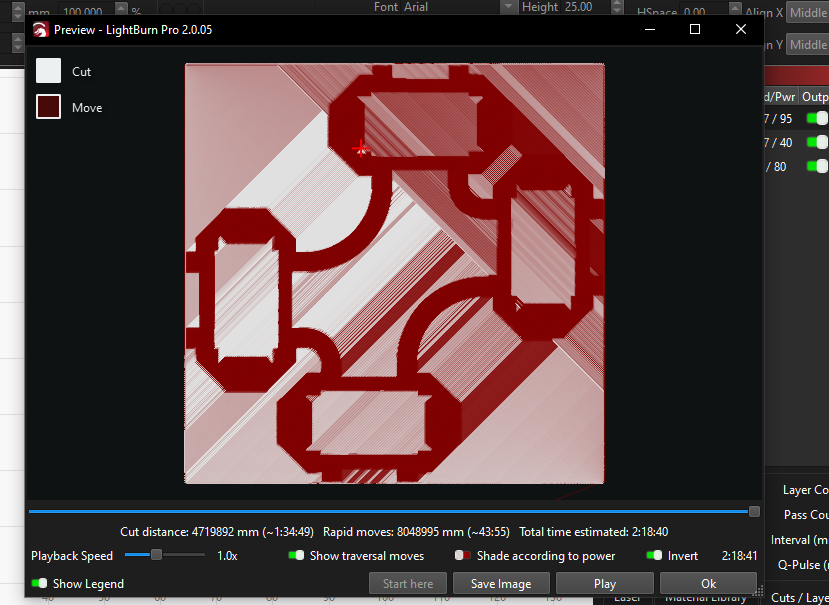
\includegraphics[width=0.6\textwidth]{figures/fillMode2.png}
    \caption{Gravação invertida no Preview.}
    \label{fig:label}
\end{figure}


Feito isso, basta definir os parâmetros e camadas no menu Cuts/Layers, utilizar o Frame no menu Laser para verificar se a gravação está no local correto e, então, começar a gravar na opção Start.


\begin{figure}[H]
    \centering
    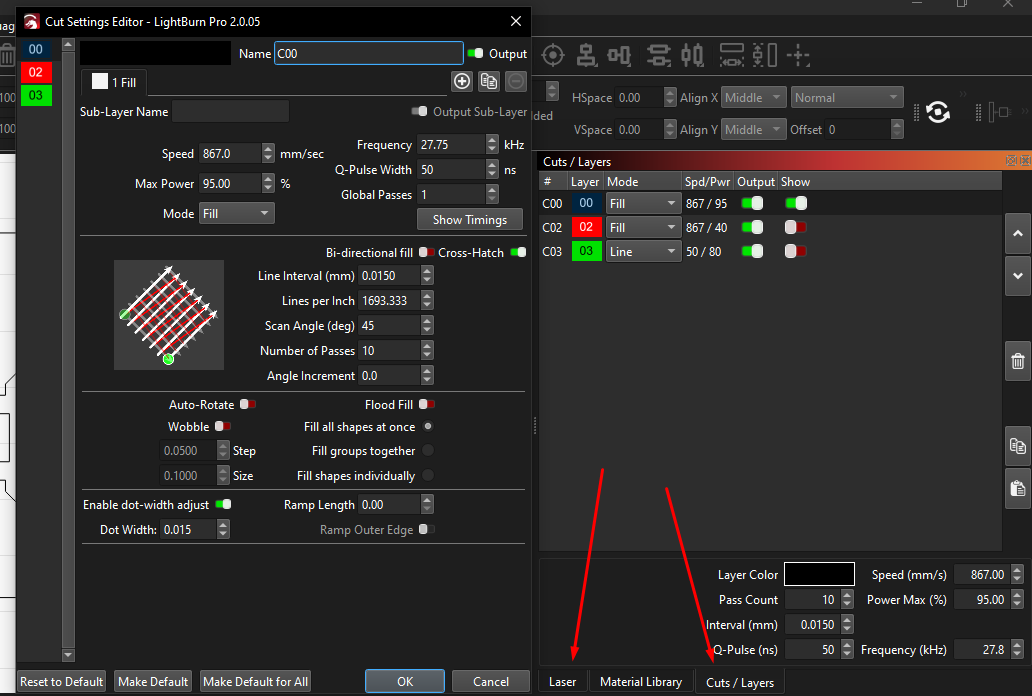
\includegraphics[width=0.6\textwidth]{figures/ParametersLayersLaser.png}
    \caption{Menu Cuts/Laser e Parameters.}
    \label{fig:label}
\end{figure}

\subsection{Camadas}
Para definir uma geometria em uma camada distinta, basta seleciona-lá e clicar em uma das 31 camadas na parte inferior do LightBurn(de 1 até 29, T1 e T2). Camadas distintas podem possuir parâmetros distintos. Assim sendo, conseguimos, por exemplo, gravar uma placa, fazer o acabamento dela e recortar ela sem ter que reconfigurar os parâmetros toda hora. Geralmente, utiliza-se o modo Fill para gravação de geometrias preenchidas e o modo Line para recortar a placa. Ou seja, o modo Fill remove o exterior(ou interior) da geometria como um todo, enquanto o modo Line apenas traça o \textit{outline} da geometria em si. 
\begin{figure}[H]
    \centering
    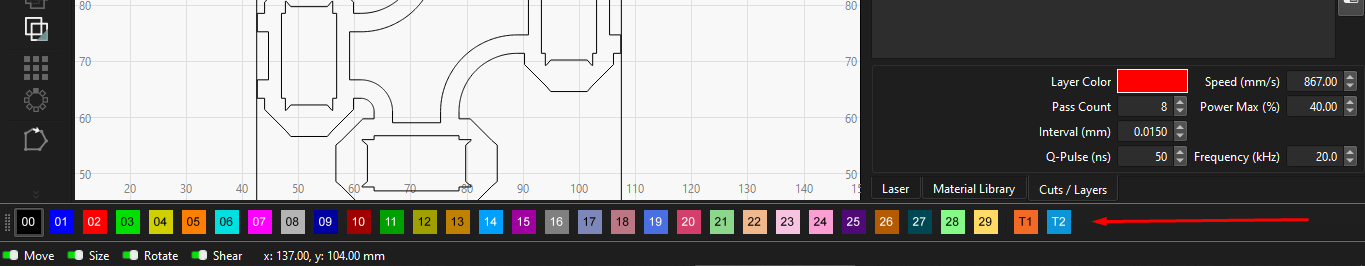
\includegraphics[width=0.6\textwidth]{figures/Layers.png}
    \caption{Camadas na parte inferior do Lightburn.}
    \label{fig:label}
\end{figure}
\subsection{Parâmetros}
Ao definir uma geometria para uma certa camada, defini-se seus parâmetros clicando duas vezes na camada. Também, é possível alterar o modo da camada, Fill, Line, ou Offset Fill(a princípio não usado), na opção "Mode". Podemos escolher se a geometria será mostrada na área de trabalho do Lightburn por meio da opção  Show e, por fim, escolher se a camada será gravada ou não por meio do Output(é possível ter uma camada listada nas Layers mas escolher não gravar ela desabilitando o Output, por exemplo).

Normalmente, define-se os parâmetros para um dado material e um dado tipo de gravação(corte, gravação), e então salva-se esses parâmetros em um arquivo de configuração que aparece na aba "Material Library". 

Caso queira salvar um conjunto de parâmetros, selecione a camada que possui os parâmetros, vá na aba Material Library e clique em Create New From Layer. 

Para designar um conjunto de parâmetros para uma camada, selecione-a, vá na aba Material Library, clique no parâmetro e então em Assign.

Para carregar ou salvar um conjunto de parâmetros, na aba Material Library, clique em Manage Library e então em Load Library ou Save Library respectivamente. 

\section{Monitoramento}
O monitoramento deve ser feito com a tampa do gabinete fechada e utilizando os óculos próprios da ComMarker para evitar danos à visão. Em hipótese alguma abra o gabinete e manipule qualquer coisa em seu interior com a gravadora em funcionamento. Limpe a lente sempre com um pano liso e limpo. 
    

\section{Manutenção Básica}
Após cada gravação, tanto o gabinete quanto a gravadora em si devem ser limpos com álcool isopropílico assegurando que nenhuma poeira/resquícios de gravação fiquem na gravadora/em seus arredores.


\section{Critérios de Qualidade da Impressão}
Os critérios de qualidade variam a depender de qual será a utilização da placa, mas sempre se concentram ao redor das bordas do material que foi removido e se houve queima do material ao redor de onde foi gravado ou por baixo(substrato, por exemplo). O ideal é que as bordas acabem de forma mais abrupta possível, sem resquícios. É ideal, também, que não haja queima qualquer ao redor do material removido ou por baixo.

\begin{figure}[H]
    \centering
    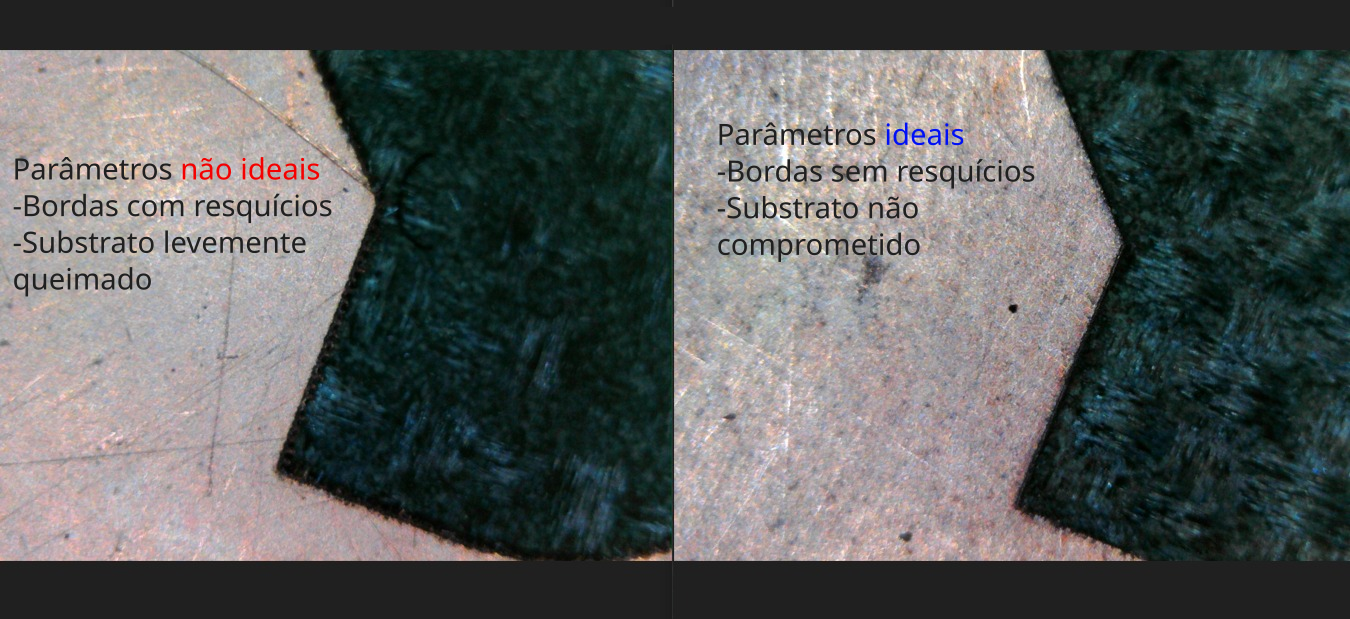
\includegraphics[width=0.6\textwidth]{figures/parametrosRuimseBons.png}
    \caption{Comparação entre parâmetros não ideais e ideais resultando em uma gravação ruim/boa.}
    \label{fig:label}
\end{figure}

 

%%%%%%%%%%%%%%%%%%%%%%%%%%%%%%%%%%%%%%%%
\nocite{*}
\printbibliography

\end{document}

